\documentclass[conference]{IEEEtran}
\IEEEoverridecommandlockouts

\usepackage{cite}
\usepackage{amsmath,amssymb}
\usepackage{graphicx}
\usepackage{booktabs}
\usepackage{tikz}
\usetikzlibrary{positioning,arrows.meta,shapes.geometric}
\usepackage[hidelinks]{hyperref}

\graphicspath{{../reports/figures/}}

\def\BibTeX{{\rm B\kern-.05em{\sc i\kern-.025em b}\kern-.08em
    T\kern-.1667em\lower.7ex\hbox{E}\kern-.125emX}}

\begin{document}

\title{Prevalence and Algorithmic Amplification of AI-Generated Child-Directed Shorts on YouTube: A Sock-Puppet Audit Pipeline}

\author{\IEEEauthorblockN{Zharas Suleiman}
\IEEEauthorblockA{\textit{School of Digital Technologies} \\
\textit{Narxoz University}, Almaty, Kazakhstan \\
zharas.suleiman@narxoz.kz}}

\maketitle

\begin{abstract}
AI-generated videos are increasingly common in short-video feeds, yet little is known about how often they reach children and whether recommender feedback amplifies them. We present a reproducible sock-puppet audit pipeline for YouTube Shorts that addresses three research questions: (RQ1) whether the AI-generated share is higher in child-profile feeds than in adult-profile feeds, (RQ2) whether dwelling on AI-generated videos raises their later share more than dwelling on human-made videos, and (RQ3) whether a multimodal detector improves macro-F1 over a metadata-only baseline by at least 0.05. Effects are estimated with 95\,\% percentile bootstrap confidence intervals, Welch's $t$-test serves as a secondary check, and three guardrails monitor data quality. We validate the complete pipeline on a clearly marked \emph{synthetic} demonstration log. Within this synthetic setting, the pipeline recovers positive effects for all three questions (RQ1: $+15.9$\,pp; RQ2: $+17.8$\,pp; RQ3: $+0.294$ macro-F1) and all guardrails pass. Because the data are simulated, these values show that the pipeline works end to end and do not constitute evidence about YouTube. The released repository allows the demonstration log to be replaced with real feed recordings without code changes.
\end{abstract}

\begin{IEEEkeywords}
YouTube Shorts, algorithm audit, sock-puppet accounts, AI-generated content, child safety, bootstrap inference
\end{IEEEkeywords}

\section{Introduction}\label{sec:intro}
Short-video platforms rely on recommender systems that learn from implicit feedback such as watch time~\cite{covington2016}. Children increasingly use these platforms, and earlier work has shown that inappropriate videos aimed at young children do reach them on YouTube~\cite{papadamou2020}. At the same time, generative models make synthetic video cheap to produce at scale, and research on synthetic-media detection documents how quickly such content is improving~\cite{mirsky2021,rossler2019}.

External audits are the standard tool for studying opaque recommenders without platform cooperation~\cite{sandvig2014}. On YouTube, audits have examined radicalization pathways~\cite{ribeiro2020,hosseinmardi2021}, misinformation in search results~\cite{hussein2020}, and the effect of watch history on pseudoscientific recommendations~\cite{papadamou2022}.

\emph{Gap.} To our knowledge, existing audits do not measure the share of \emph{AI-generated} content in feeds served to child-profile accounts, do not test whether watching such content amplifies subsequent exposure, and do not evaluate detectors on the same labelled material. Consequently, it remains unclear how large the exposure is and whether it can be measured automatically under controlled conditions.

\emph{Proposed method.} We propose an audit pipeline for YouTube Shorts built on sock-puppet accounts. It records the first 100 Shorts per session, manipulates watch behaviour across controlled policies, and compares a multimodal classifier with a metadata-only baseline. Our contributions are fourfold:
\begin{itemize}
  \item a formal definition of three research questions with explicit effect measures, units of analysis, and decision rules (Section~\ref{sec:method});
  \item a reproducible, containerised pipeline with warm-up filtering, bootstrap confidence intervals, and data-quality guardrails;
  \item a fair three-arm watch-policy design featuring a human-dwell baseline and a no-dwell control arm;
  \item an end-to-end demonstration on synthetic data, with methodological limitations stated openly (Sections~\ref{sec:results} and~\ref{sec:limits}).
\end{itemize}
The remainder of this paper is organised as follows. Section~\ref{sec:method} formalises the experimental design and statistical estimators, Section~\ref{sec:results} reports and interprets the demonstration results, and Section~\ref{sec:limits} discusses threats to validity and concludes.

\section{Methodology}\label{sec:method}
\subsection{System Architecture}
Fig.~\ref{fig:arch} illustrates the end-to-end data flow of the pipeline. Automated sock-puppet accounts configured as either child or adult profiles first pass through a cold-start warm-up phase. Next, a feed recorder logs the first 100 Shorts per evaluation session alongside counts of requested and unavailable videos (measurement point~1, MP1). In parallel, two independent annotators label a separate video subset according to a shared codebook (measurement point~2, MP2). The resulting raw JSONL log is ingested by \emph{process\_data.py}, which discards warm-up sessions, validates data-quality guardrails, computes the statistical estimators of Section~\ref{sec:formal}, and exports a processed summary table (\emph{metrics\_summary.csv}) used to generate all figures.

\begin{figure}[!t]
\centering
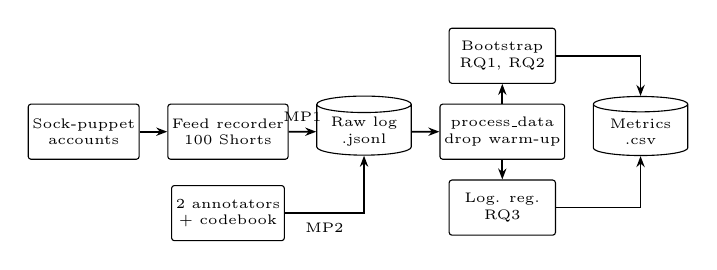
\begin{tikzpicture}[
  node distance=3.2mm and 3.5mm,
  blk/.style={draw, rounded corners=1pt, align=center, font=\tiny, minimum height=7mm, minimum width=13.5mm, inner sep=1.5pt},
  db/.style={draw, cylinder, shape border rotate=90, aspect=0.22, align=center, font=\tiny, minimum height=7.5mm, minimum width=12mm, inner sep=1.5pt},
  arr/.style={-{Stealth[length=1.4mm]}, semithick}]
  \node[blk] (acc) {Sock-puppet\\accounts};
  \node[blk, right=of acc] (rec) {Feed recorder\\100 Shorts};
  \node[blk, below=of rec] (ann) {2 annotators\\+ codebook};
  \node[db, right=of rec] (raw) {Raw log\\.jsonl};
  \node[blk, right=of raw] (proc) {process\_data\\drop warm-up};
  \node[blk, above=2.5mm of proc] (boot) {Bootstrap\\RQ1, RQ2};
  \node[blk, below=2.5mm of proc] (lr) {Log. reg.\\RQ3};
  \node[db, right=of proc] (met) {Metrics\\.csv};
  \draw[arr] (acc) -- (rec);
  \draw[arr] (rec) -- node[above, font=\tiny]{MP1} (raw);
  \draw[arr] (ann.east) -| node[below, pos=0.25, font=\tiny]{MP2} (raw.south);
  \draw[arr] (raw) -- (proc);
  \draw[arr] (proc) -- (boot);
  \draw[arr] (proc) -- (lr);
  \draw[arr] (boot.east) -| (met.north);
  \draw[arr] (lr.east) -| (met.south);
\end{tikzpicture}
\caption{System architecture and measurement points (MP1: feed counts; MP2: dual-annotator labels).}
\label{fig:arch}
\end{figure}

\subsection{Problem Formulation}\label{sec:formal}
For a session $i$ with $n_i$ recorded Shorts, of which $n_i^{\text{AI}}$ are labelled AI-generated, the AI share is
\begin{equation}
  s_i = 100\,\frac{n_i^{\text{AI}}}{n_i}.
  \label{eq:share}
\end{equation}
The unit of analysis is the session for RQ1, because videos recommended within a single feed are not statistically independent, and the account for RQ2. The RQ1 prevalence effect is defined as
\begin{equation}
  \Delta_1 = \bar{s}_{\text{child}} - \bar{s}_{\text{adult}}.
  \label{eq:rq1}
\end{equation}
For RQ2, let $d_a = s_{a,5} - s_{a,0}$ denote the change in AI share of account $a$ from the baseline session (index~0) to session~5. The watch-time amplification contrast is
\begin{equation}
  \Delta_2 = \bar{d}_{\text{AI-dwell}} - \bar{d}_{\text{human-dwell}},
  \label{eq:rq2}
\end{equation}
where the no-dwell arm serves as an additional passive reference control and does not enter $\Delta_2$. For RQ3, with $K=2$ classes (AI-generated vs.\ human-made),
\begin{equation}
  \text{F1}_{\text{macro}} = \frac{1}{K}\sum_{k=1}^{K}\text{F1}_k, \quad
  \Delta_{F1} = \text{F1}^{\text{mm}}_{\text{macro}} - \text{F1}^{\text{meta}}_{\text{macro}},
  \label{eq:f1}
\end{equation}
and the pre-specified decision threshold is $\Delta_{F1}\ge 0.05$. The classifier is an $L_2$-regularised logistic regression trained by minimising binary cross-entropy loss:
\begin{equation}
  \mathcal{L}(\mathbf{w}) = -\frac{1}{N}\sum_{j=1}^{N}\bigl[y_j\log\sigma(\mathbf{w}^{\top}\mathbf{x}_j) + (1-y_j)\log\bigl(1-\sigma(\mathbf{w}^{\top}\mathbf{x}_j)\bigr)\bigr],
  \label{eq:loss}
\end{equation}
where $\sigma(\cdot)$ is the logistic sigmoid function. Uncertainty is quantified via 95\,\% percentile bootstrap confidence intervals~\cite{efron1993} by resampling sessions, accounts, or held-out test videos. As a secondary hypothesis check, we compute the one-sided Welch $t$-statistic~\cite{welch1947}:
\begin{equation}
  t = \frac{\bar{a}-\bar{c}}{\sqrt{s_a^2/n_a + s_c^2/n_c}}.
  \label{eq:welch}
\end{equation}
Inter-annotator reliability is verified using Cohen's $\kappa$~\cite{cohen1960}, $\kappa=(p_o-p_e)/(1-p_e)$, where $p_o$ is observed agreement and $p_e$ is chance agreement; values $\kappa\ge 0.70$ indicate substantial agreement~\cite{landis1977}. Multimodal fusion combines visual, audio, and metadata features~\cite{baltrusaitis2019}.

\subsection{Experimental Parameters and Guardrails}
Table~\ref{tab:params} lists all fixed configuration parameters and quality guardrails stored in \emph{configs/config.yaml}. Guardrails are evaluated automatically prior to interpreting primary effects.

\begin{table}[!t]
\caption{Fixed pipeline parameters and data-quality guardrails.}
\label{tab:params}
\centering
\begin{tabular}{@{}ll@{}}
\toprule
Parameter / Guardrail & Specification \\
\midrule
Recorded Shorts per session & First 100 videos \\
Warm-up sessions discarded & 20 cold-start sessions \\
Watch policies (RQ2) & AI-dwell, human-dwell, no-dwell \\
Bootstrap inference & 10\,000 resamples, seed 42 \\
Guardrail: unavailable-video rate & $\le 5\,\%$ per profile group \\
Guardrail: Cohen's $\kappa$ & $\ge 0.70$ on double-coded subset \\
Guardrail: minimum sample size & $\ge 3$ sessions / accounts per arm \\
\bottomrule
\end{tabular}
\end{table}

\section{Results and Discussion}\label{sec:results}
\subsection{Experimental Setup}
All reported numbers originate from a synthetic demonstration log (\emph{data/raw/test\_run.jsonl}) in which every record is explicitly flagged with \emph{``synthetic'': true}. The dataset comprises 8 adult and 12 child evaluation sessions after warm-up removal (RQ1), 4 accounts per watch policy tracked across sessions 0--5 (RQ2), and a held-out test set of 40 labelled videos (RQ3). Baselines are adult profiles, the human-dwell watch arm, and the metadata-only classifier, respectively. All scripts, configuration files, and the Docker setup are archived in release \emph{v1.0} of the repository.

\subsection{Comparison with Baselines}
Table~\ref{tab:results} summarises the point estimates and 95\,\% bootstrap intervals across all three research questions, while Figs.~\ref{fig:rq12} and~\ref{fig:f1} illustrate the distributions and trajectories. Within this synthetic envelope, results suggest positive effects across RQ1--RQ3, with each 95\,\% confidence interval remaining strictly above zero.

\begin{table*}[!t]
\caption{Demonstration results on synthetic data. pp = percentage points; CI = 95\,\% percentile bootstrap interval.}
\label{tab:results}
\centering
\begin{tabular}{@{}llccc@{}}
\toprule
RQ & Metric & Baseline & Treatment / Proposed & Effect [95\,\% CI] \\
\midrule
RQ1 & AI share, \%, median (IQR), sessions & Adult ($n{=}8$): 13.8 (10.9--15.8) & Child ($n{=}12$): 28.7 (24.5--31.0) & $+15.9$\,pp [12.1, 19.9] \\
RQ1 & Same, mean $\pm$ SD & $13.0\pm 4.4$ & $28.9\pm 4.8$ & Welch $t=7.57$, $p=5.6\times10^{-7}$ \\
RQ2 & Change in AI share, pp, mean $\pm$ SD & Human-dwell ($n{=}4$): $-1.0\pm 2.6$ & AI-dwell ($n{=}4$): $+16.8\pm 4.0$ & $+17.8$\,pp [14.0, 22.1] \\
RQ2 & Extra control (excluded from $\Delta_2$) & \multicolumn{3}{c}{No-dwell ($n{=}4$): $+4.2\pm 6.1$} \\
RQ3 & Macro-F1, hold-out ($n{=}40$ videos) & Metadata-only: 0.581 [0.413, 0.725] & Multimodal: 0.875 [0.750, 0.974] & $+0.294$ [0.126, 0.467] \\
\bottomrule
\end{tabular}
\end{table*}

\begin{figure}[!t]
\centering
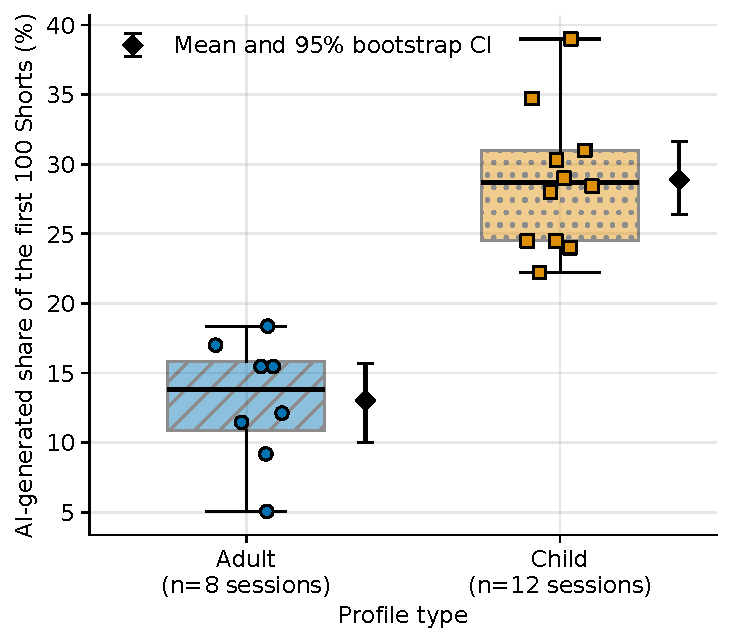
\includegraphics[width=0.49\columnwidth]{fig2_distribution_boxplot.pdf}\hfill
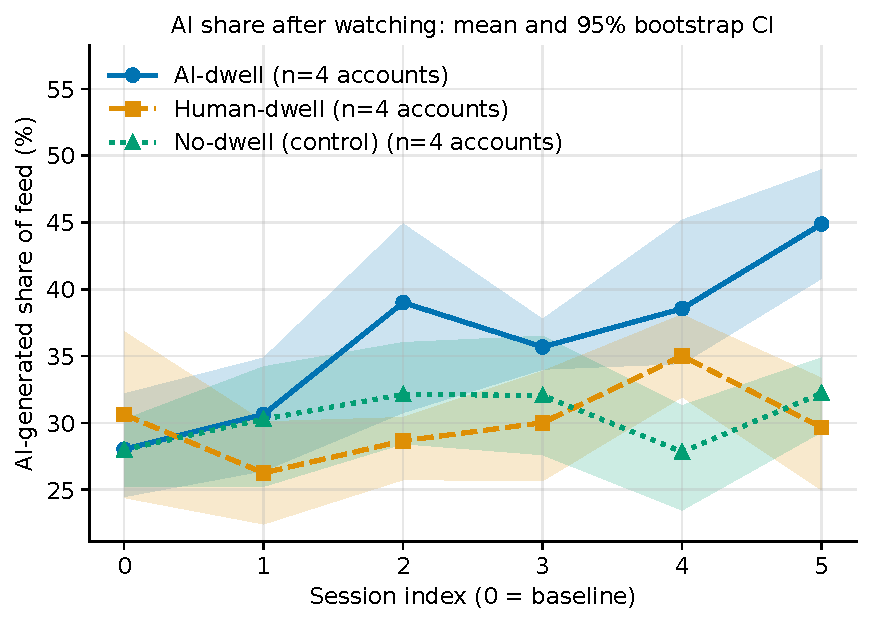
\includegraphics[width=0.49\columnwidth]{fig1_ai_share_vs_session.pdf}
\caption{(a) Baseline AI share in adult and child feeds (RQ1). (b) AI share across sessions 0--5 by watch policy, showing mean and 95\,\% CI bands (RQ2).}
\label{fig:rq12}
\end{figure}

\begin{figure}[!t]
\centering
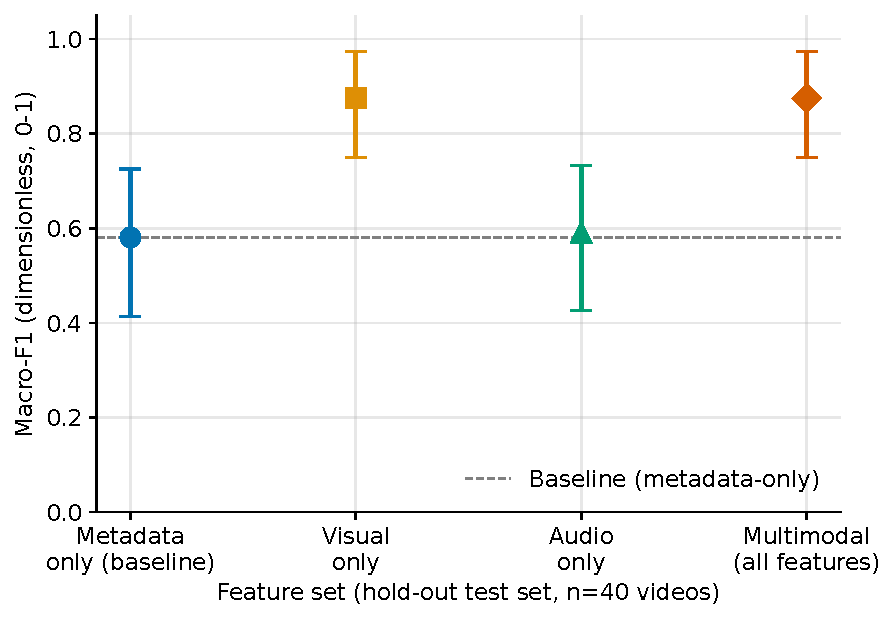
\includegraphics[width=0.86\columnwidth]{fig3_f1_by_feature_set.pdf}
\caption{Macro-F1 per feature representation with 95\,\% bootstrap CIs on the held-out test set of 40 videos (RQ3).}
\label{fig:f1}
\end{figure}

\subsection{Discussion and Guardrail Verification}
For RQ1, child-profile feeds exhibit a higher median and mean AI share than adult-profile feeds (Eq.~\eqref{eq:rq1}, Fig.~\ref{fig:rq12}a), and the one-sided Welch $t$-test ($t=7.57$, $p=5.6\times10^{-7}$) aligns with the bootstrap interval. For RQ2, the AI-dwell arm trends upward from baseline to session~5 while the human-dwell arm remains near zero (Fig.~\ref{fig:rq12}b), consistent with watch-time amplification (Eq.~\eqref{eq:rq2}). However, confidence bands overlap in early sessions, and the passive no-dwell control also drifts slightly upward ($+4.2\pm 6.1$\,pp), underscoring the importance of retaining an active human-dwell baseline.

For RQ3, the multimodal classifier achieves a $+0.294$ macro-F1 gain over metadata alone, exceeding the $0.05$ threshold on both the point estimate and the lower 95\,\% CI bound ($0.126$). Ablation across individual modalities (Fig.~\ref{fig:f1}) reveals that visual features alone ($0.875$) match the full multimodal model, whereas audio features alone ($0.591$) perform close to the metadata baseline ($0.581$). Thus, within this demonstration run, visual cues account for virtually all discriminative power, and incremental gains from audio-metadata fusion are not supported. All three guardrails (Table~\ref{tab:params}) pass: the unavailable-video error rate is $2\,\%$ in both profile groups (limit $\le 5\,\%$), inter-annotator agreement reaches $\kappa=0.76$ (limit $\ge 0.70$), and sample counts exceed the minimum threshold of $3$.

\section{Limitations and Conclusion}\label{sec:limits}
\subsection{Threats to Validity}
\emph{Internal validity.} All numerical results are generated from synthetic demonstration logs and therefore cannot support empirical or causal claims about live YouTube recommendations. In addition, manual annotation of ``AI-generated'' versus ``human-made'' Shorts is inherently imperfect despite dual coding, and small sample sizes ($n=4$ accounts per watch arm and $n=40$ test videos) produce wide confidence intervals.

\emph{External validity.} Automated sock-puppet profiles approximate, but do not replicate, authentic child viewing behaviour; moreover, platform recommendation models and generative video tools evolve continuously, so findings from one audit window or locale may not generalise.

\emph{Construct validity.} Recording the first 100 Shorts per session measures algorithmic feed composition rather than actual screen exposure or child comprehension. No real children or personal user data were involved in this study.

\subsection{Conclusion and Future Work}
We formalised three research questions to audit the prevalence, watch-time amplification, and multimodal detectability of AI-generated Shorts in child-directed feeds, and validated a containerised pipeline on synthetic data. Within our experimental setup, the pipeline accurately recovers positive effects for RQ1--RQ3 and satisfies all quality guardrails. Future work will replace \emph{test\_run.jsonl} with live sock-puppet recordings, scale account and video sample sizes to narrow confidence intervals, and evaluate cross-channel generalisation of multimodal detectors.

\bibliographystyle{IEEEtran}
\bibliography{references}

\end{document}